\title{Signs of Bipolar Disorder in Social Media Text}

\author{Ivan Sekulić\\
Mentor: Nikos Gianniotis\\
}%\footnotesize{March 11, 2019}}

\institute[]{
Natural Language Processing Group}

%\date{\today}

\begin{frame}
  \titlepage
\end{frame}

\begin{frame}
  \frametitle{Motivation}
  \centering
  How does everyday language reflect basic social and personality processes?
\end{frame}

\begin{frame}
  \frametitle{Motivation}
  \centering
  How does everyday language reflect our mental health?
\end{frame}

\begin{frame}
  \frametitle{Meet Fynn}
  \begin{tabular}{cl}  
    \begin{tabular}{c}
        
\includegraphics[height=6cm, width=4cm,keepaspectratio]{fig/businessman-607834_1280.png}
    \end{tabular}
    & \begin{tabular}{l}
        \parbox{0.5\linewidth}{
        \begin{itemize}
            \item In a bad mood, stays in bed the whole weekend
            \pause
            \item Goes out with friends next week
            \pause
            \item Relatable?
        \end{itemize}
    }
    \end{tabular}  \\
    \end{tabular}
\end{frame}

\begin{frame}{Meet Sophie}
\begin{tabular}{cl}  
         \begin{tabular}{c}
           
\includegraphics[height=6cm, width=4cm,keepaspectratio]{fig/teacher-359311_1280.png}
           \end{tabular}
           & \begin{tabular}{l}
             \parbox{0.5\linewidth}{%  change the parbox width as appropiate
             \begin{itemize}
      \item Struggling to get out of bed for months
      \pause
      \item Diagnosed with depression
      \pause
      \item 10 days of sleep deprivation, unease, traveling and money spending
  \end{itemize}
    }
         \end{tabular}  \\
\end{tabular}
    
\end{frame}

\begin{frame}
  \frametitle{Bipolar disorder}
  \begin{center}
    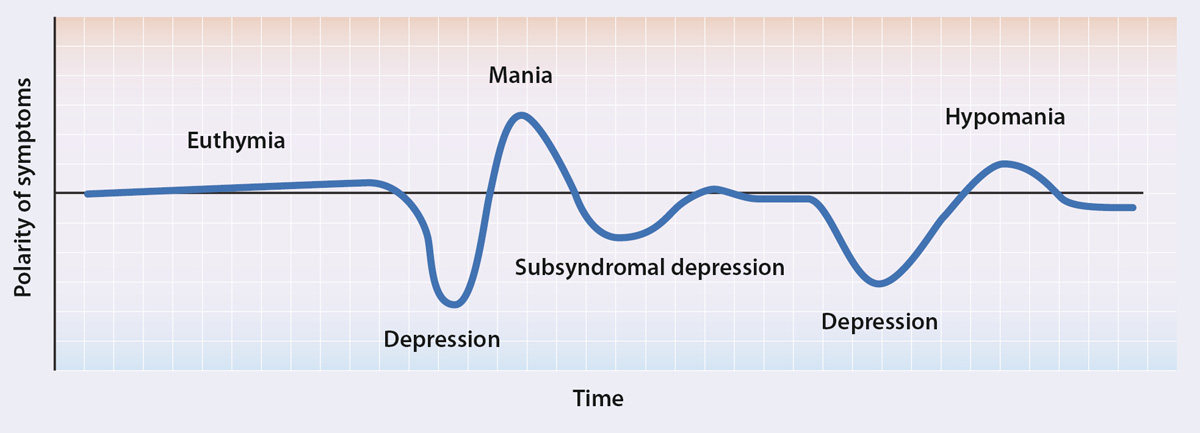
\includegraphics[width=\textwidth,height=0.7\textheight,keepaspectratio]{fig/bipolar-img1.jpg}
  \end{center}


\begin{itemize}
    \item Recurrent manic and depressive episodes
    \item Affects 60M people worldwide, 6\% suicide rate
\end{itemize}
  
\end{frame}

\begin{frame}
  \frametitle{Where is NLP?}
  Imagine Sophie and Fynn write \textbf{blogs}, or they \textbf{tweet}, or are active \textbf{Redditors}
  \begin{center}
  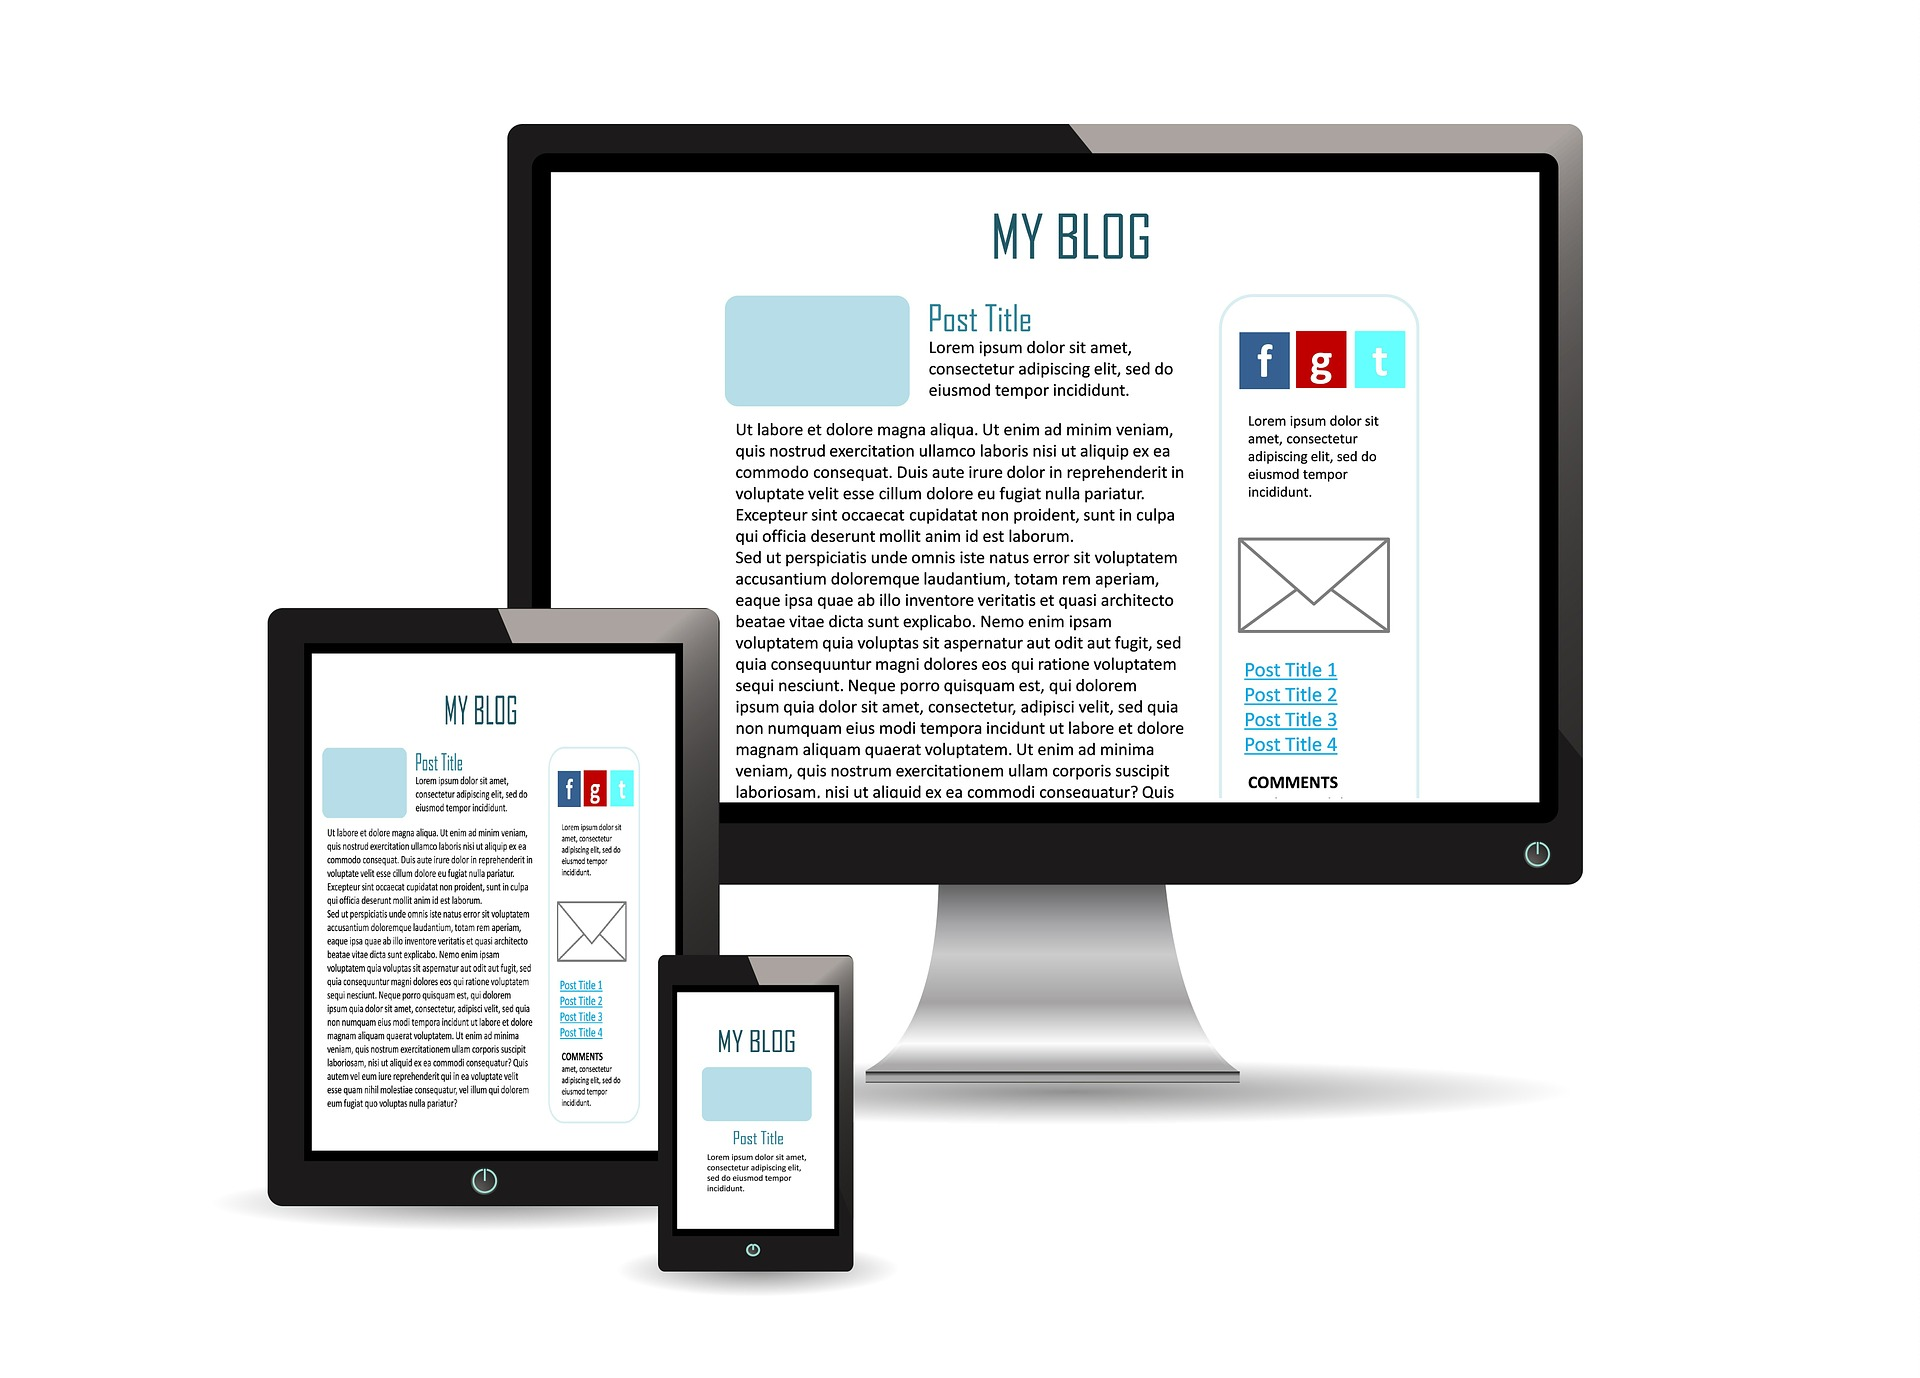
\includegraphics[width=120,height=100, keepaspectratio]{fig/blog.jpg}
  
\includegraphics[width=90,height=90, keepaspectratio]{fig/twitter1.png}
  \hspace{3cm}
  
\includegraphics[width=90,height=90, keepaspectratio]{fig/reddit1.png}
  \end{center}
\end{frame}

\begin{frame}
  \frametitle{How can NLP help?}
  \centering
  \begin{itemize}
    \item Early detection
    \begin{itemize}
        \item Discover potential disorder from author's text
        \item Timely reaction $\rightarrow$ Suicide prevention
    \end{itemize}
    \pause
    \item Understand how illnesses manifest in language
    \begin{itemize}
        \item Evaluate contemporary psychological theories % models, perspectives
       % \item Provide a new perspective for psychologists
        \item Make large-scale text analysis available to psychologists\\
        $\rightarrow$ \textbf{~3.5k Reddit users with bipolar disorder}
    \end{itemize}

  \end{itemize}
\end{frame}


\begin{frame}
  \frametitle{Fynn's language vs Sophie's language}
  Compared to control group, authors with bipolar disorder tend differ in:
  \begin{itemize}
    \item \emph{I-talk} -- in line with research on depression
    \item \emph{affect} -- increased usage of affect-related words
    \item \emph{health} -- talk more about health-related topics
    \item \emph{pronoun usage} -- reflects standings in social hierarchies
    \item ...
  \end{itemize}
\end{frame}

\begin{frame}
  \frametitle{Bipolar disorder prediction}
  \begin{adjustwidth}{-1.5em}{-1.5em}
      \begin{tabular}{lll}
           
\includegraphics[width=100, height=100,keepaspectratio]{fig/documents.jpg}
           & \raisebox{10mm}[0pt][0pt]{\makebox[80][c]{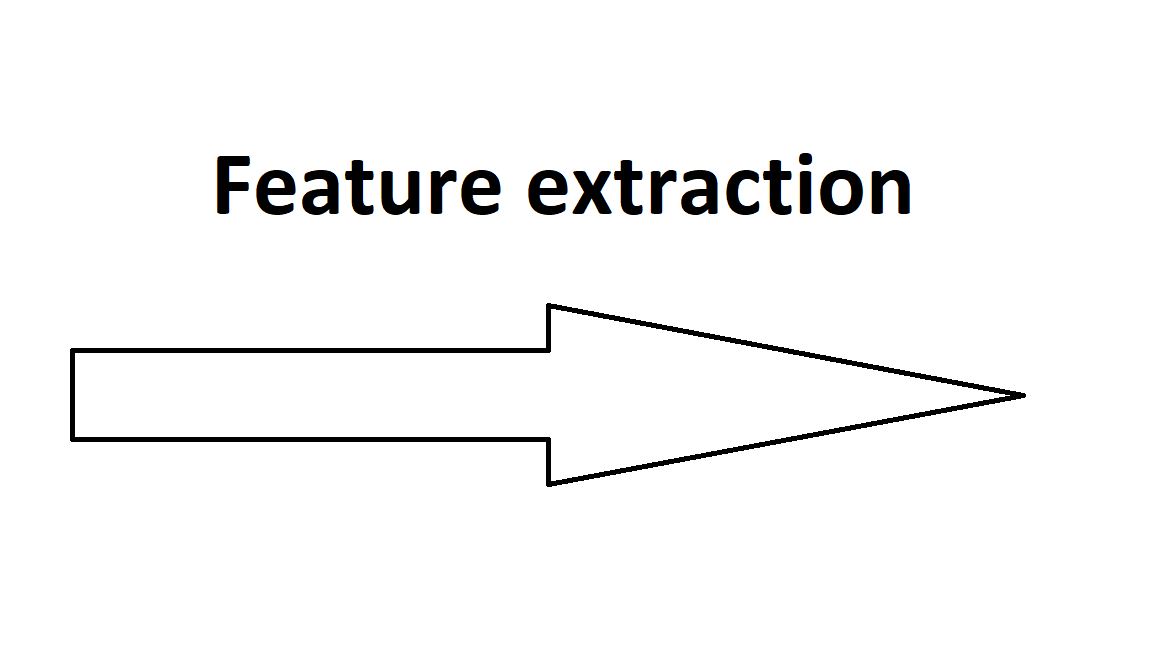
\includegraphics[width=80,height=80,keepaspectratio]{fig/fe2.png}}}



           & 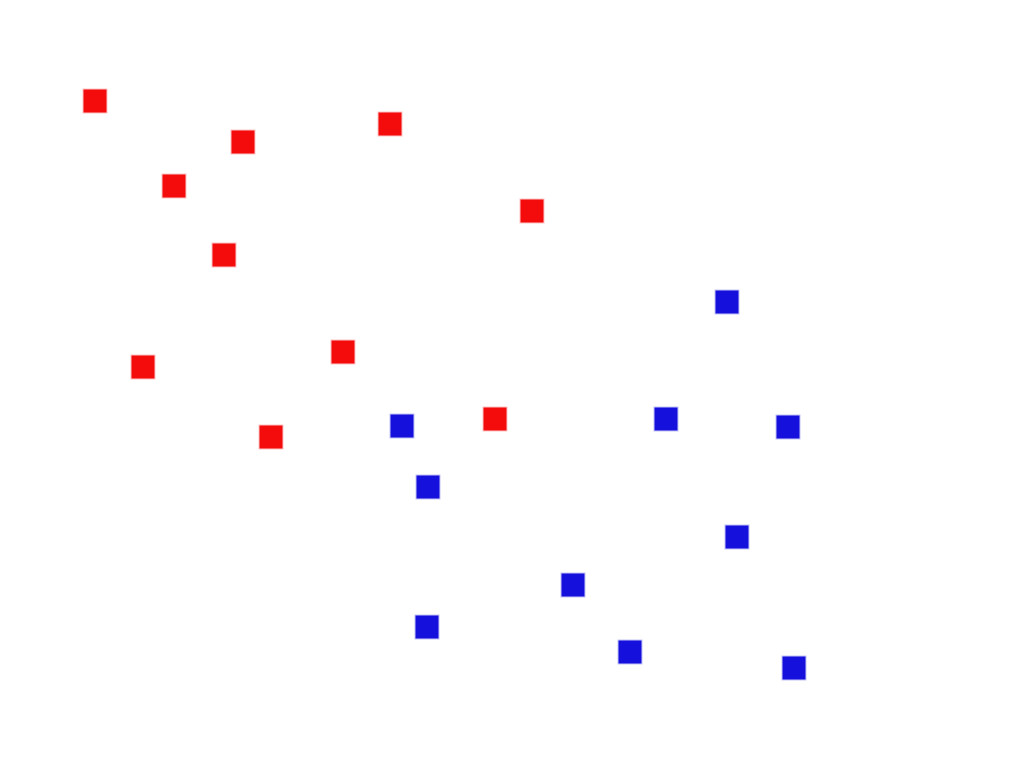
\includegraphics[width=130, height=130,keepaspectratio]{fig/inspace.jpg}
    \end{tabular}
    \end{adjustwidth}
\end{frame}

\begin{frame}
  \frametitle{Bipolar disorder prediction}
  \begin{adjustwidth}{-1.5em}{-1.5em}
      \begin{tabular}{lll}
           
\includegraphics[width=100, height=100,keepaspectratio]{fig/documents.jpg}
           &  \raisebox{10mm}[0pt][0pt]{\makebox[80][c]{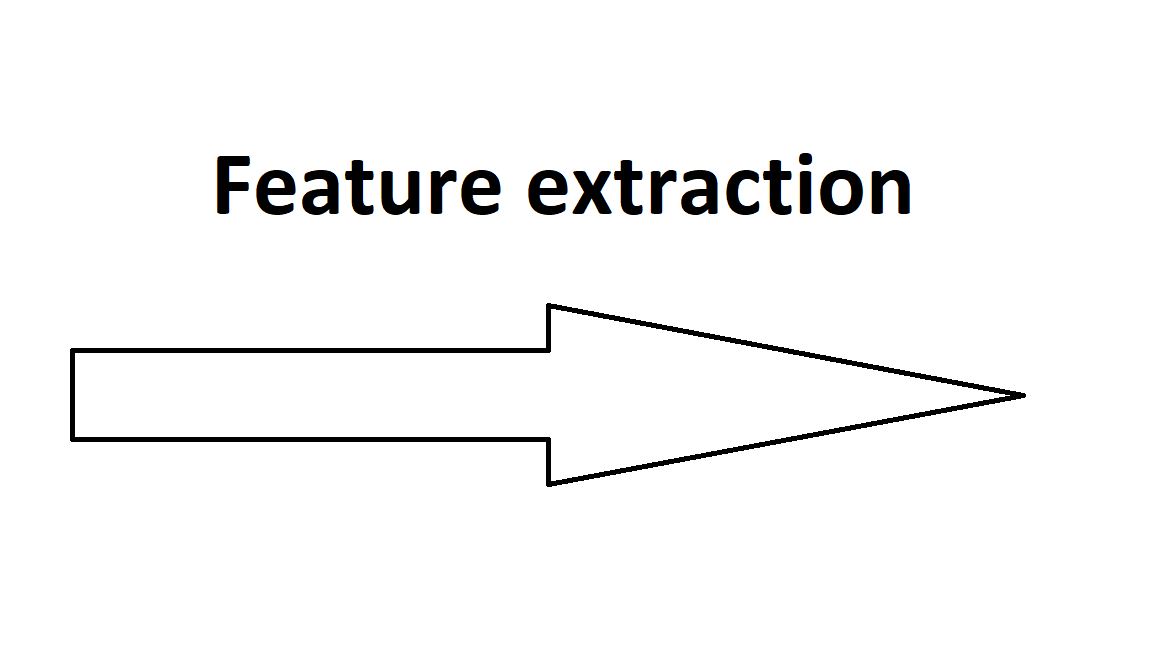
\includegraphics[width=80,height=80,keepaspectratio]{fig/fe2.png}}}
           & 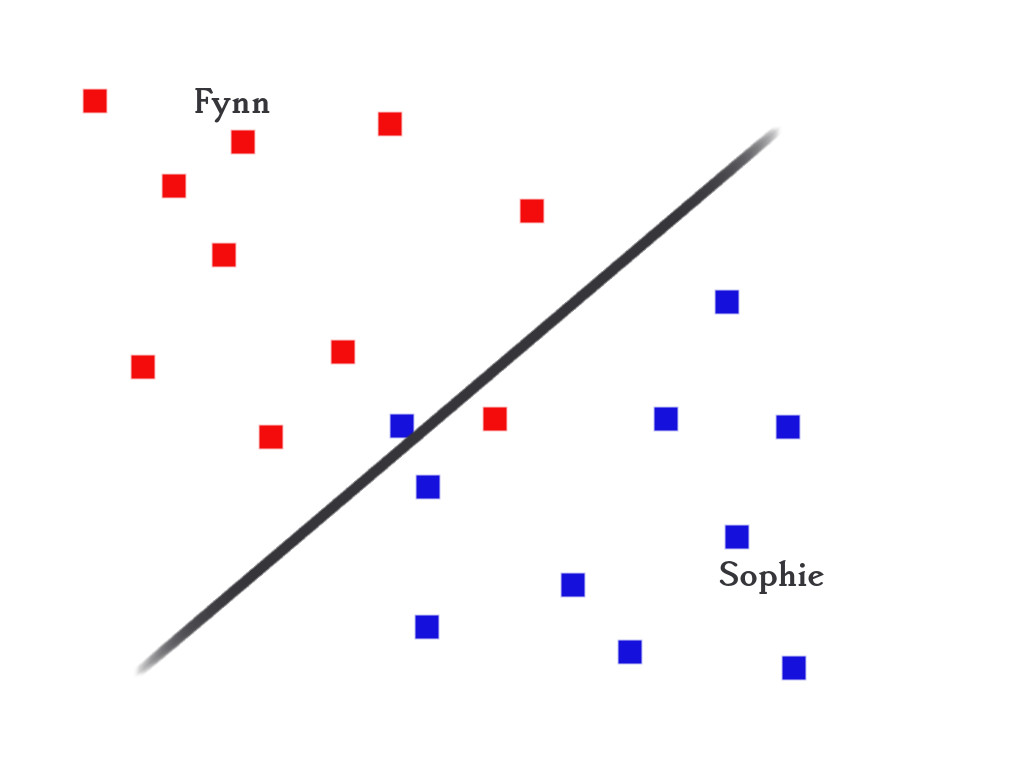
\includegraphics[width=130, height=130,keepaspectratio]{fig/clf2.jpg}
    \end{tabular}

    \begin{center}
        \large{Binary classification task: \textbf{86\% accuracy}}
    \end{center}
    
    \end{adjustwidth}
\end{frame}

\begin{frame}
  \frametitle{Time component}
  \begin{itemize}
      \item By aggregating all of user's text, we can't understand how bipolar disorder progresses in time
      \pause
      \item Goal: detect when manic and depressive episodes occur
  \end{itemize}

  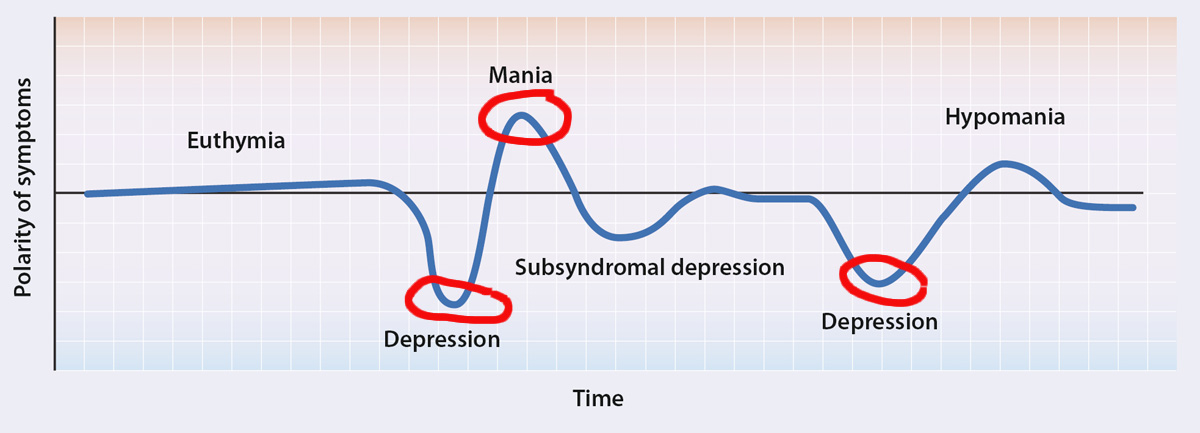
\includegraphics[width=\textwidth,height=0.5\textheight,keepaspectratio]{fig/bipolar-circled.jpg}
\end{frame}

\begin{frame}{Progression through time}

Group comments by day, week, or month
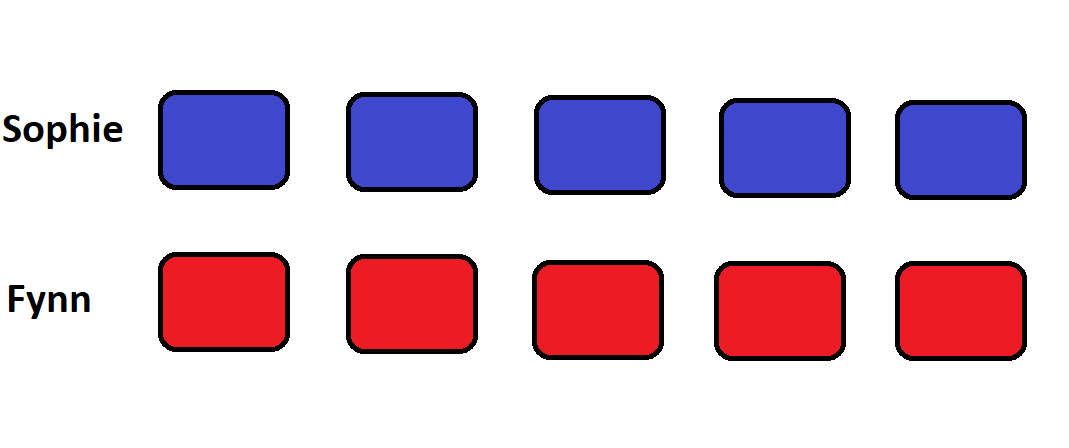
\includegraphics[width=300,height=200,keepaspectratio]{fig/obojano_malo.png}

    Higher \textbf{variance} of emotion-related features in bipolar group:
    \begin{itemize}
        \item \textbf{affect, positive emotions, negative emotions, anxiety, sadness}
    \end{itemize}   
\end{frame}

\begin{frame}
  \frametitle{Work in progress}
  \begin{itemize}
    \item Supervised classification: \textbf{Time-aware} vs \textbf{time-agnostic} models
    \item Detecting manic and depressive episodes
    \begin{itemize}
        \item Semi-supervised: One-class classification
        \item Unsupervised: autoencoders for time-series
    \end{itemize}

  \end{itemize}
\end{frame}

\begin{frame}
  \centering
  \huge{Thank you!}
\end{frame}

